% !TEX root = ../main.tex

% Background section

\section{Verifying Variational Boosting's Effectiveness} \label{sec:verify}
In this section, we use a mixture of two bivariate normal distributions as an example target distribution to verify and critique the effectiveness of the VB algorithm, as well as the two practical considerations. We begin by looking at the weighted EM initialization. From \cref{fig:fail}, we see that when approximating $\pi(x) = 0.5 N\left(\begin{bmatrix} 2\\2 \end{bmatrix}, I_2\right) + 0.5N\left(\begin{bmatrix} -2\\-2 \end{bmatrix}, I_2\right)$ indeed fails to capture the second mode. In fact, the weight of the second component, initialized through the weighted EM approach with a sample size $40$, is exactly zero. While the intuition the weighted EM approach makes sense, it relies on some of the samples from the current mixture approximation producing unlikely samples. Specifically, after we have found the first mode in \cref{fig:fail}, all of the sampled observations of the current approximation stays within the mode that is already well-approximated. Then whether we can jump out of this local mode depends on that some of the samples to be used in the weighted EM algorithm comes from the edge of the already-found mode or further away from the mode. As the variance of the first component decreases, it becomes more and more unlikely that we can jump out of this local mode using the weighted EM approach. While it is a difficult problem to tackle, perhaps some improvements need to be done on the weighted EM approach for it to be more reliable.\\\\
Discarding this component initialization, if initialization works in the target distribution's favour, as shown in \cref{fig:success}, we indeed can very effectively approximate the posterior distribution. It is worth noting that a tiny $0.1$ covariance has been added to the posterior in \cref{fig:success}. However, even with just a diagonal covariance structure, the posterior approximation is still very close to the target distribution, hence confirming the intuition on selecting the structure to be imposed on the covariance matrix.

\begin{figure}[H]
\centering
\begin{subfigure}{0.45\textwidth}
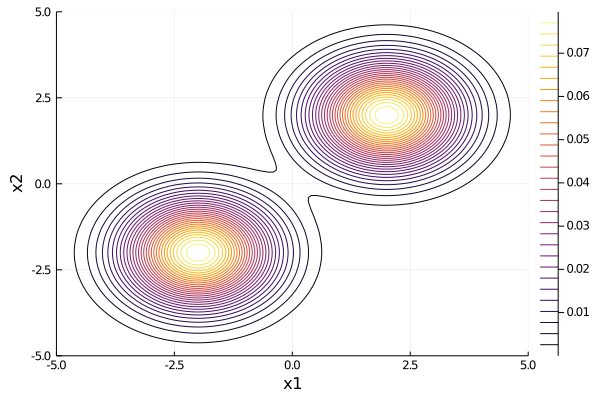
\includegraphics[width=1\linewidth]{../../plot/true_post_far.png}
\caption{True posterior distritbution}
\end{subfigure}
\begin{subfigure}{0.45\textwidth}
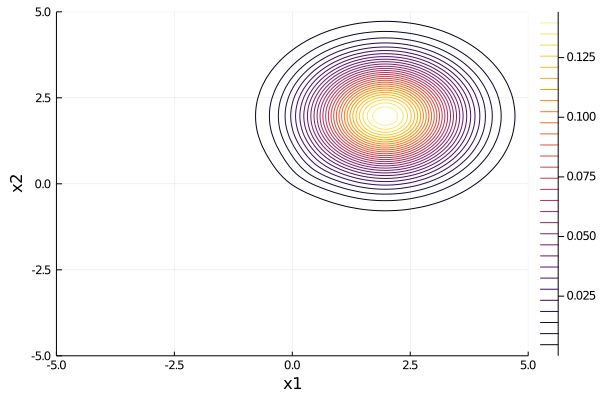
\includegraphics[width=1\linewidth]{../../plot/approx_post_far.png}
\caption{Variational boosting approximating with two components}
\end{subfigure}
\caption{Comparing the target distribution and the variational boosting approximation using the weighed EM component initialization.}
\label{fig:fail}
\end{figure}

\begin{figure}[H]
\centering
\begin{subfigure}{0.45\textwidth}
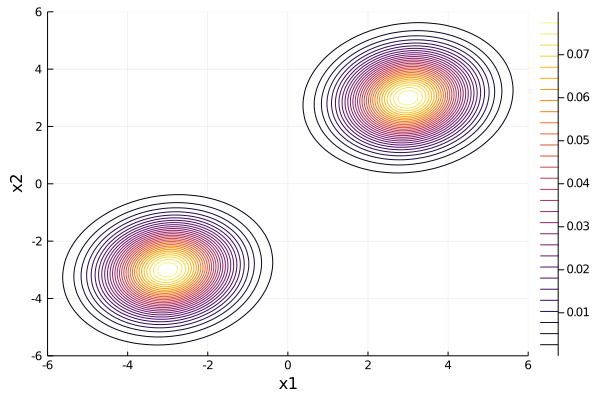
\includegraphics[width=1\linewidth]{../../plot/true_post_close.png}
\caption{True posterior distritbution}
\end{subfigure}
\begin{subfigure}{0.45\textwidth}
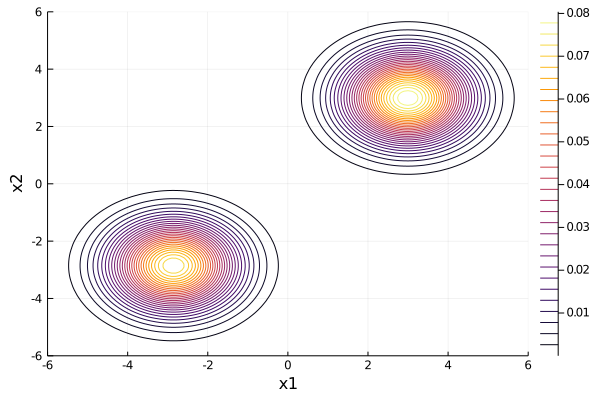
\includegraphics[width=1\linewidth]{../../plot/approx_post_close.png}
\caption{Variational boosting approximating with two components (diagonal covariance)}
\end{subfigure}
\caption{Comparing the target distribution and the variational boosting approximation without the weighed EM component initialization.}
\label{fig:success}
\end{figure}
% ...